\section{Relativistic Doppler Effect}

\makelabheader %(Space for student name, etc., defined in master.tex)

\begin{center}
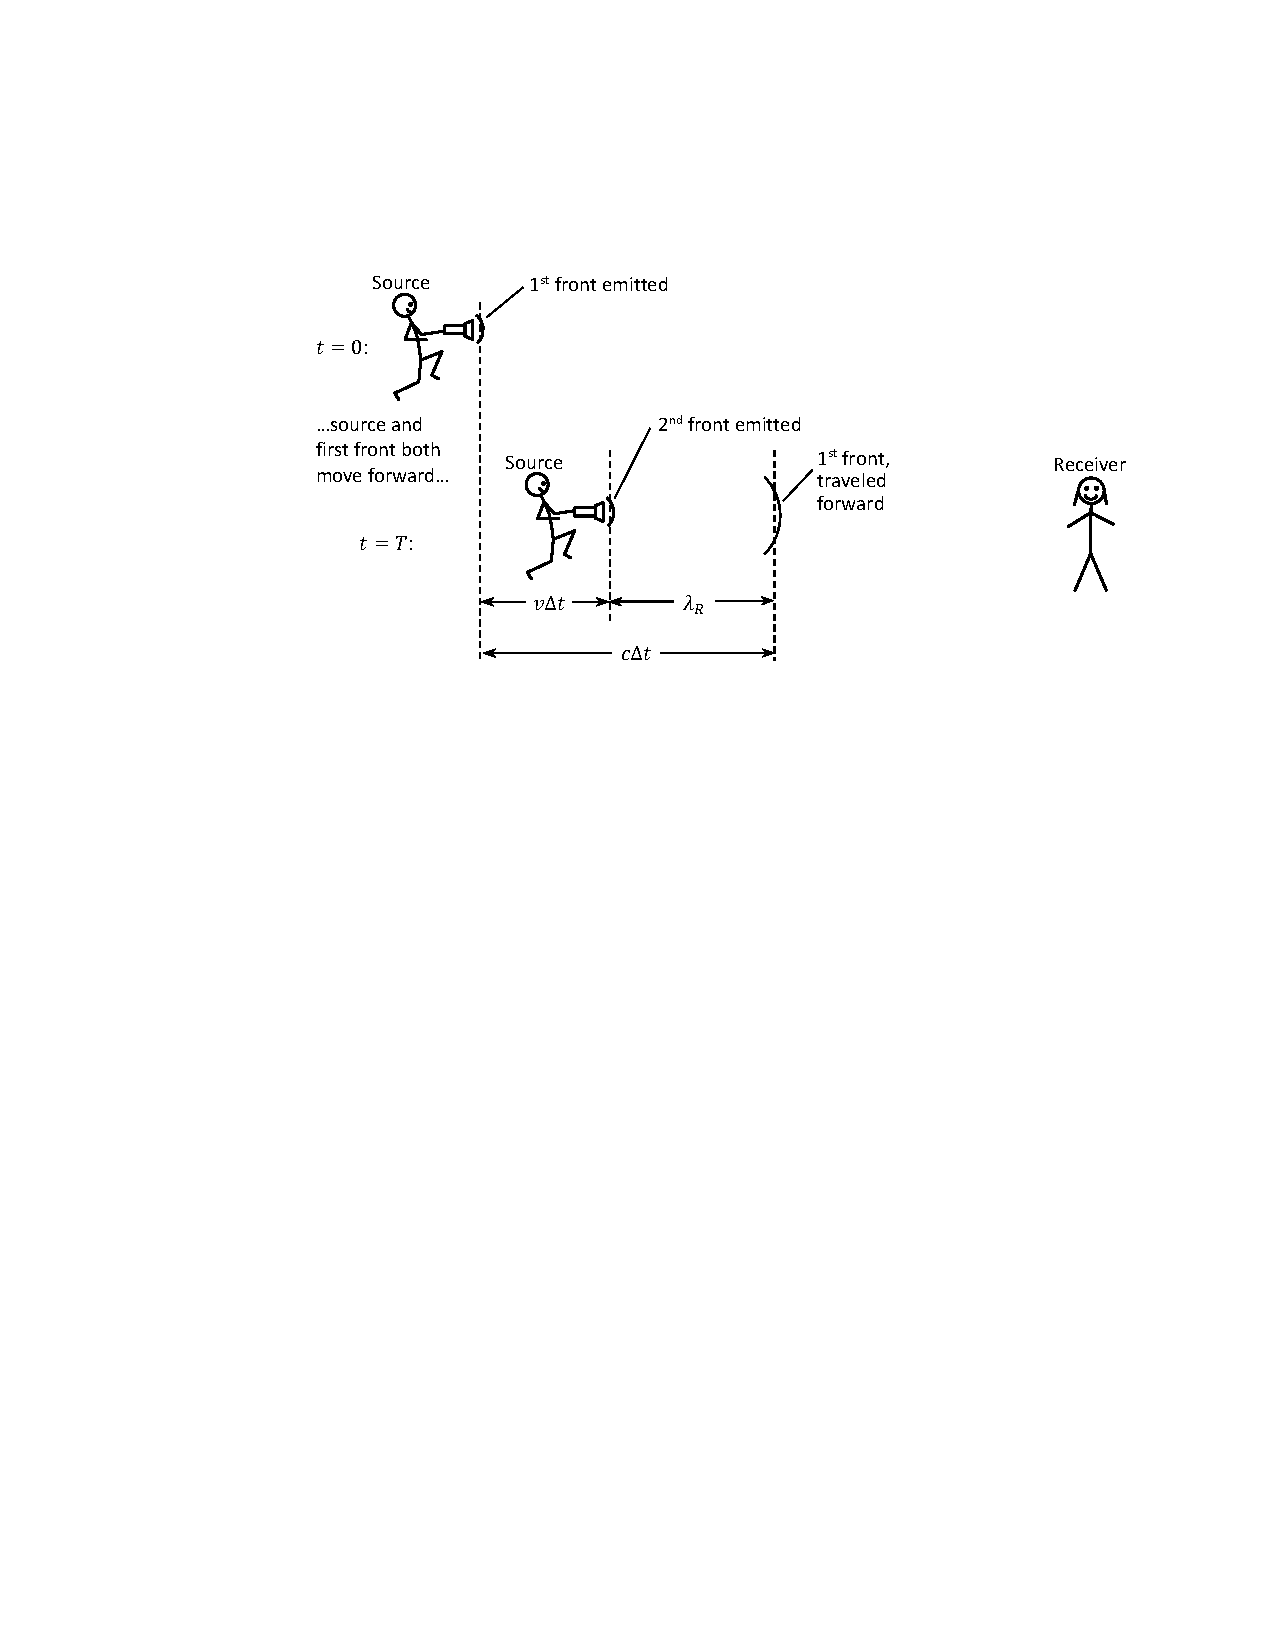
\includegraphics[width=0.75\textwidth]{relativistic_doppler/relativistic_front_motion.pdf}
\end{center}

\textbf{Activity 1: Moving Source, Fixed Receiver}

Your friend (the ``source'') is shining a flashlight while running towards you at a very fast speed $v$.  The first wavefront is emitted at time $t=0$.

\begin{enumerate}[labparts]
\item After one period $\Delta t=T$, the first wavefront emitted has traveled a distance $c\Delta t$ and the source has traveled a distance $v\Delta t$.  What is the wavelength $\lambda_R$ seen by the receiver?  (Answer in $v$, $c$, and $\Delta t$.)
\answerspace{0.3in}

\item Using the relationship between $f_R$, $\lambda_R$, and $c$, write the frequency $f_R$ seen by the receiver  in terms of $v$, $c$, and $\Delta t$.
\answerspace{0.3in}

\item Who measures the proper time $\Delta t_0$ between the two fronts being emitted?
\answerspace{0.3in}

\item Using the relationship that $f_S=1/\Delta t_0$, write the time $\Delta t$ in terms of the frequency $f_S$ measured by the source and the Lorentz factor $\gamma_v$.
\answerspace{0.3in}

\item Combine your answer in (d) above and your previous expression for $f_R$ to get $f_R$ in terms of $f_S$, $v$, $c$, and $\gamma_v$.
\answerspace{0.8in}

\pagebreak[3]

\item Rewrite $\gamma_v$ in your expression above as $\gamma_v = \left(\sqrt{1 - v^2/c^2} \right)^{-1}$, and then rewrite your previous answer for $f_R$ in terms of only $f_S$ and $\beta$, where $\beta = v/c$.
\answerspace{0.8in}

\item Use the identity that $1 - \beta^2 = (1 + \beta)(1 - \beta)$ to simplify your expression for $f_R$ above.
\answerspace{1.0in}

\item You derived your expression for $f_R$ above by assuming that the source was moving and the receiver was at rest.  Bearing in mind the basic tenets of relativity, does it matter which one is moving?

\end{enumerate}

\vfill

Note our sign convention here:
\begin{align*}
\textrm{positive } \beta &\Longrightarrow \textrm{motion towards each other (``approaching'')} \\
\textrm{negative } \beta &\Longrightarrow \textrm{motion away from each other (``receding'')} 
\end{align*}
